\documentclass[../main.tex]{subfiles}

\addbibresource{\subfix{../references.bib}}

\begin{document}

\ifSubfilesClassLoaded{%
    \setcounter{chapter}{7}%
    \begin{refsection}
}{}

\chapter{Basic Block Identification dan Local Optimization}
\label{chap:basic-block}

\begin{subcpmk}
  \item \textbf{Sub-CPMK 4.2:} Mengimplementasikan basic block identification
\end{subcpmk}

% ============================================================
% MATERI POKOK
% ============================================================
\section{Dasar Basic Block dan Karakteristiknya}

\compiler{Basic Block} adalah sekumpulan instruksi kode antara (\textit{intermediate code}) yang dieksekusi secara berurutan tanpa adanya instruksi lompatan (\textit{jump/branch}) di tengah-tengahnya.

\subsection{Definisi Formal}
Sebuah blok instruksi disebut \textit{Basic Block} jika:
\begin{itemize}
    \item Hanya memiliki satu titik masuk (\textit{entry point}), yaitu instruksi pertama.
    \item Hanya memiliki satu titik keluar (\textit{exit point}), yaitu instruksi terakhir.
    \item Semua instruksi di dalamnya dieksekusi secara sekuensial.
\end{itemize}

\subsection{Contoh Basic Block}
Perhatikan potongan kode berikut:
\begin{lstlisting}
t1 = a + b
t2 = t1 * c
x = t2
\end{lstlisting}
Setelah eksekusi dimulai dari baris pertama, semua baris berikutnya dijamin akan dieksekusi secara berurutan. Ini adalah satu \textit{Basic Block}.

\section{Algoritma Identifikasi Leader}

Untuk membagi kode antara menjadi beberapa \textit{basic block}, kita harus mengidentifikasi instruksi-instruksi yang menjadi "pemimpin" (\textit{leader}).

\subsection{Aturan Identifikasi Leader}
Instruksi adalah \textit{leader} jika memenuhi salah satu syarat berikut:
\begin{enumerate}
    \item Instruksi pertama dalam program/fungsi.
    \item Instruksi yang merupakan target dari sebuah lompatan (\textit{conditional jump} atau \textit{unconditional jump}).
    \item Instruksi yang muncul tepat setelah instruksi lompatan.
\end{enumerate}

\subsection{Pembentukan Blok}
Setelah semua \textit{leader} ditemukan, setiap \textit{basic block} terdiri dari sebuah \textit{leader} dan semua instruksi berikutnya hingga (tapi tidak termasuk) instruksi \textit{leader} berikutnya.

\begin{figure}[!htbp]
    \centering
    \adjustbox{max width=0.8\textwidth,center}{%
    \begin{tikzpicture}[
        inst/.style={rectangle, draw=blue!50, fill=blue!10, font=\tiny, align=left},
        arrow/.style={->, >=stealth, thick}
    ]
    \node[inst] (i1) {L1: leader 1\\instr 2\\if ... goto L2};
    \node[inst, below=1cm of i1] (i2) {L2: leader 2\\instr 4\\return};
    \draw[arrow] (i1) -- node[right, font=\tiny] {Branch} (i2);
    \end{tikzpicture}%
    }
    \caption{Identifikasi leader dan pembentukan blok}
\end{figure}

\section{Local Optimization: Folding dan Simplification}

Optimasi lokal bekerja hanya di dalam satu \textit{basic block}. Tujuannya adalah mengurangi beban komputasi instruksi aritmatika tanpa perlu menganalisis seluruh program.

\subsection{1. Constant Folding}
Jika semua operan bersifat konstan, kompilator melakukan perhitungan saat itu juga.
\begin{itemize}
    \item \textbf{Sebelum}: \code{x = 2 * 3.14 * r}
    \item \textbf{Sesudah}: \code{x = 6.28 * r}
\end{itemize}

\subsection{2. Algebraic Simplification}
Menggunakan identitas matematika untuk menghapus operasi yang tidak perlu (\textit{Identity Elimination}).
\begin{itemize}
    \item \code{x + 0} $\to$ \code{x}
    \item \code{x * 1} $\to$ \code{x}
    \item \code{x / 1} $\to$ \code{x}
\end{itemize}

\subsection{3. Strength Reduction}
Mengganti operasi yang "mahal" (berat bagi CPU) dengan operasi yang "murah" namun ekuivalen. Biasanya dilakukan untuk perkalian dan pembagian dengan pangkat 2.
\begin{enumerate}
    \item \textbf{Multiplication}: \code{x * 2} diganti \code{x + x} atau \code{x << 1}.
    \item \textbf{Division}: \code{x / 4} diganti \code{x >> 2}.
    \item \textbf{Exponent}: \code{pow(x, 2)} diganti \code{x * x}.
\end{enumerate}

\begin{figure}[!htbp]
    \centering
    \adjustbox{max width=0.8\textwidth,center}{%
    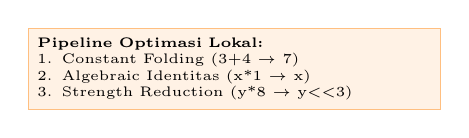
\begin{tikzpicture}[
        rect/.style={rectangle, draw=orange!50, fill=orange!10, text width=5cm, font=\tiny}
    ]
    \node[rect] (opt) {
        \textbf{Pipeline Optimasi Lokal:}\\
        1. Constant Folding (3+4 $\to$ 7)\\
        2. Algebraic Identitas (x*1 $\to$ x)\\
        3. Strength Reduction (y*8 $\to$ y<<3)
    };
    \end{tikzpicture}%
    }
    \caption{Hierarki Optimasi Lokal pada Ekspresi Aritmatika}
\end{figure}

\section{Representasi DAG untuk Optimasi Lokal}

\textit{Directed Acyclic Graph} (\compiler{DAG}) adalah struktur data yang sangat kuat untuk menganalisis aliran data di dalam sebuah \textit{basic block}.

\subsection{Manfaat DAG}
Mengubah deretan instruksi ke dalam bentuk DAG memberikan beberapa keuntungan otomatis bagi kompilator:
\begin{enumerate}
    \item \textbf{Common Subexpression Elimination}: Jika sebuah perhitungan (misal \code{a + b}) muncul lebih dari sekali, DAG secara otomatis hanya akan membuat satu node untuk hasil tersebut.
    \item \textbf{Dead Code Elimination}: Node yang tidak memiliki label variabel keluar (output) dan tidak digunakan oleh node lain dapat langsung dihapus.
    \item \textbf{Instruction Reordering}: Struktur graf memungkinkan kompilator menata ulang instruksi tanpa merusak ketergantungan data.
\end{enumerate}

\subsection{Algoritma Konstruksi DAG}
Setiap instruksi TAC \texttt{x = y op z} diproses sebagai berikut:
\begin{enumerate}
    \item Cari node untuk operan \texttt{y} dan \texttt{z}. Jika belum ada, buat node daun (\textit{leaf}).
    \item Periksa apakah sudah ada node dengan operator \texttt{op} yang memiliki anak \texttt{y} dan \texttt{z}.
    \item Jika ada, beri label \texttt{x} pada node tersebut (hasil penggunaan kembali).
    \item Jika tidak ada, buat node baru dengan operator \texttt{op}, hubungkan ke \texttt{y} dan \texttt{z}, lalu beri label \texttt{x}.
\end{enumerate}

\begin{figure}[!htbp]
    \centering
    \adjustbox{max width=0.8\textwidth,center}{%
    \begin{tikzpicture}[
        node/.style={circle, draw=blue!50, fill=blue!10, minimum size=0.8cm, font=\small},
        arrow/.style={->, >=stealth, thick}
    ]
    % DAG for a = b+c; d = b+c
    \node[node] (plus) at (0,0) {+};
    \node[node] (b) at (-1,-1.5) {b};
    \node[node] (c) at (1,-1.5) {c};
    \draw[arrow] (plus) -- (b);
    \draw[arrow] (plus) -- (c);
    
    \node[right=0.2cm of plus, font=\small] {\{a, d\}};
    \node[below=1.8cm of plus, font=\itshape\footnotesize, text width=5cm, align=center] {
        Satu node '+' melayani variabel 'a' dan 'd'. Hilangkan redundansi.
    };
    \end{tikzpicture}%
    }
    \caption{Representasi DAG untuk Eliminasi Subekspresi Umum}
\end{figure}

\section{Control Flow Graph (CFG) Construction}

\compiler{Control Flow Graph (CFG)} adalah representasi berarah di mana setiap \textit{node} adalah sebuah \textit{basic block} dan setiap \textit{edge} menunjukkan kemungkinan aliran kendali antar blok tersebut.

\subsection{Membangun Tepi (Edges)}
Sebuah tepi ditambahkan dari blok $B_1$ ke blok $B_2$ jika:
\begin{itemize}
    \item Terdapat instruksi lompatan (jump) dari akhir $B_1$ ke awal $B_2$.
    \item $B_2$ terletak tepat setelah $B_1$ dalam urutan program, dan $B_1$ tidak diakhiri dengan lompatan mutlak (\textit{unconditional jump}).
\end{itemize}

\subsection{Pentingnya CFG}
CFG adalah struktur data utama untuk melakukan \textit{Global Optimization} dan analisis aliran data (\textit{Data Flow Analysis}) yang mencakup seluruh fungsi/program.

\begin{figure}[!htbp]
    \centering
    \adjustbox{max width=0.8\textwidth,center}{%
    \begin{tikzpicture}[
        block/.style={rectangle, draw=green!50, fill=green!10, font=\tiny, align=center},
        arrow/.style={->, >=stealth, thick}
    ]
    \node[block] (b1) {Block 1 (Entry)};
    \node[block, below left=1cm of b1] (b2) {Block 2 (True)};
    \node[block, below right=1cm of b1] (b3) {Block 3 (False)};
    \node[block, below=2.5cm of b1] (b4) {Block 4 (Exit)};
    \draw[arrow] (b1) -- (b2);
    \draw[arrow] (b1) -- (b3);
    \draw[arrow] (b2) -- (b4);
    \draw[arrow] (b3) -- (b4);
    \end{tikzpicture}%
    }
    \caption{Contoh Control Flow Graph sederhana}
\end{figure}


% ============================================================
% AKTIVITAS PEMBELAJARAN
% ============================================================
\begin{aktivitas}
  \item \textbf{Block Identification}: Implementasikan algoritma basic block identification.
  \item \textbf{CFG Construction}: Bangun control flow graph dari three-address code.
  \item \textbf{Local Optimizations}: Implementasikan constant folding dan algebraic simplification.
  \item \textbf{Data Flow}: Implementasikan reaching definitions analysis.
  \item \textbf{Optimization Pipeline}: Buat pipeline untuk multiple local optimizations.
\end{aktivitas}

% ============================================================
% LATIHAN DAN REFLEKSI
% ============================================================
\begin{latihan}
  \item Identifikasi basic blocks dalam potongan three-address code yang diberikan!
  \item Gambarkan CFG untuk program dengan nested if-else dan while loops!
  \item Implementasikan constant folding untuk ekspresi aritmatika kompleks!
  \item Analisis reaching definitions untuk program sederhana!
  \item Identifikasi dead code yang dapat dieliminasi!
  \item \textbf{Refleksi}: Bagaimana basic blocks menyederhanakan optimasi compiler?
\end{latihan}

% ============================================================
% ASESMEN
% ============================================================
\begin{asesmen}
\textbf{Instrumen Penilaian untuk Sub-CPMK 4.2}

\textbf{A. Pilihan Ganda}

\begin{enumerate}
  \item Basic block memiliki:
  \begin{enumerate}
    \item Multiple entry points
    \item Single entry point
    \item Multiple exit points
    \item No exit points
  \end{enumerate}
  
  \item Leader adalah instruksi yang:
  \begin{enumerate}
    \item Pertama dalam program
    \item Target dari jump
    \item Setelah conditional jump
    \item Semua jawaban benar
  \end{enumerate}
  
  \item Constant folding adalah:
  \begin{enumerate}
    \item Menghapus konstanta
    \item Menggabungkan konstanta
    \item Mengidentifikasi konstanta
    \item Mengoptimasi loops
  \end{enumerate}
\end{enumerate}

\textbf{B. Essay}

\begin{enumerate}
  \item Jelaskan algoritma basic block identification dengan contoh konkret!
  \item Implementasikan local optimization pipeline dengan constant folding, copy propagation, dan dead code elimination!
\end{enumerate}

\textbf{Rubrik Penilaian}: Lihat Lampiran A
\end{asesmen}

% ============================================================
% CHECKLIST KOMPETENSI
% ============================================================
\begin{checklist}
  \item Saya dapat mengimplementasikan basic block identification
  \item Saya dapat membangun control flow graph
  \item Saya dapat melakukan constant folding
  \item Saya dapat menerapkan algebraic simplification
  \item Saya dapat mengimplementasikan copy propagation
  \item Saya dapat melakukan dead code elimination
\end{checklist}

% ============================================================
% RANGKUMAN
% ============================================================
\begin{rangkuman}
Bab ini membahas basic block identification dan local optimization, termasuk algoritma identifikasi, CFG construction, dan berbagai teknik optimasi lokal. Mahasiswa belajar membangun fondasi untuk global optimizations.

\textbf{Poin Kunci:}
\begin{itemize}
  \item Basic blocks adalah unit analisis untuk optimasi compiler
  \item Leaders menandai awal dari setiap basic block
  \item CFG merepresentasikan alur kontrol antar basic blocks
  \item Local optimizations bekerja dalam satu basic block
  \item Data flow analysis menyediakan informasi untuk optimasi
\end{itemize}

\textbf{Kata Kunci}: \compiler{Basic Block}, \compiler{Control Flow Graph}, \compiler{Local Optimization}, \compiler{Constant Folding}, \compiler{Copy Propagation}, \compiler{Dead Code Elimination}, \compiler{Data Flow Analysis}
\end{rangkuman}

\ifSubfilesClassLoaded{%
    \clearpage
    \printbibliography[title={Daftar Pustaka}]
    \end{refsection}
}{}

\end{document}
